%
% File acl2016.tex
%
%% Based on the style files for ACL-2015, with some improvements
%%  taken from the NAACL-2016 style
%% Based on the style files for ACL-2014, which were, in turn,
%% Based on the style files for ACL-2013, which were, in turn,
%% Based on the style files for ACL-2012, which were, in turn,
%% based on the style files for ACL-2011, which were, in turn, 
%% based on the style files for ACL-2010, which were, in turn, 
%% based on the style files for ACL-IJCNLP-2009, which were, in turn,
%% based on the style files for EACL-2009 and IJCNLP-2008...

%% Based on the style files for EACL 2006 by 
%%e.agirre@ehu.es or Sergi.Balari@uab.es
%% and that of ACL 08 by Joakim Nivre and Noah Smith

\documentclass[11pt]{article}
\usepackage{acl2016}
\usepackage{times}
\usepackage{url}
\usepackage{latexsym}
\usepackage{graphicx}

\aclfinalcopy % Uncomment this line for the final submission
%\def\aclpaperid{***} %  Enter the acl Paper ID here

%\setlength\titlebox{5cm}
% You can expand the titlebox if you need extra space
% to show all the authors. Please do not make the titlebox
% smaller than 5cm (the original size); we will check this
% in the camera-ready version and ask you to change it back.

\newcommand\BibTeX{B{\sc ib}\TeX}

\title{Assessing a Word Similarity Model for Determining Overall Category}

\author{Ethan Campbell-Taylor \\
Linguistics '16\\\And
  Becky Marvin \\
  Cognitive Science '16 \\
  \\\And
  Harvey Xia \\
  Computer Science '16 \\}

\date{May 9, 2016}

\begin{document}
\maketitle
\begin{abstract}
  This document contains the methodology and results of a study examining the effectiveness of using WordNet's semantic hierarchy information to classify text documents. We used the semantic similarity information from WordNet, in addition to a hierarchical clustering algorithm to determine the similarity of the nouns in a given text document. We then found the hypernyms of the resulting clusters and compared the hypernyms to the labeled categories of the document. We assessed the accuracy of our algorithm by comparing its judgments of overall categories to the actual labeled categories of documents.
\end{abstract}

\section{Introduction}

Text classification has previously been researched using ``bag of words'' representations of word meanings. We explore a different approach in this paper: that of using WordNet's available semantic similarity information combined with a hierarchical clustering algorithm to determine the overall category of a text document. We believe this approach better models the semantic information in a given document, which could be useful in determining the overall category of a document.


\section{Our Model}

\subsection{The Algorithm}

Since our model is attempting to determine the category of a document based on the nouns used in it, the first step in our algorithm is to extract all the document's nouns. After removing punctuation and non-ascii characters, the algorithm tokenizes each line and tags the tokens with nltk's part of speech tagger. 

It then stems the relevant nouns, determined by whether their stemmed versions exist in wordnet. We removed the stems of words ending in ``ing,'' ``s,'' ``e,'' ``able,'' ``y,'' and ``er.'' For example, ``photography'' becomes ``photograph,'' but ``agency'' remains as is, since ``agenc'' is not recognized as a word by WordNet. After stemming, the algorithm counts every instance of each token and stores this information in a Python dictionary. For each of these tokens, the algorithm finds the corresponding synset (the set of senses listed in WordNet for the word) if it exists. These synsets are used to compute similarity measures for the purposes of clustering.

Having done this, the algorithm computes a similarity matrix for every pair of nouns in the document: that is, it calculates and stores the similarity of the synsets for each noun pair. We used the fastcluster library to do heirarchical clustering: we  exclude clusters smaller than size 2 and larger than size 99, as well as those with a distance of less than 0.5. The clusters are then sorted by size, those with the greatest number of raw tokens appearing first. Finally, for each cluster, the algorithm finds the hypernym (the least common ancestor of all the synsets in the cluster).

The algorithm evaluates performance by finding the item in the hypernyms returned by our algorithm that is most similar to a tag for each labeled tag of the text document. We use Wu-Palmer similarity as a measure of how similar two words are according to WordNet.

\section{Evaluation}

We tested our algorithm on 295 articles taken from NPR's website, since these articles contained tags describing what the article was about. On average, the articles contained about 925 words, 135 of which were nouns. Of these 135 nouns, there were on average 87 distinct nouns. These nouns were then clustered by our algorithm and the hypernyms were created for each cluster. The most similar hypernym was computed for each tag for the article, and this similarity score (which took on values from 0 to 1) was then summed for all the tags and divided by the number of tags. That is, our overall similarity score for each document was:

\[
 \frac{1}{\#_{tags}} \sum_{t \in tags}{(\max_{h \in hypernyms}{wupSimilarity(h, t)})}
\]

This score would be closer to 1 if the closest hypernym for each tag was highly similar, and closer to 0 if the closest hypernym for each tag was highly dissimilar.

\section{Results}

We computed these similarity scores explained above for each article, and the resulting distribution of scores for each article is shown in Figure \ref{scoreHist}

\begin{figure*}[t]
\centering
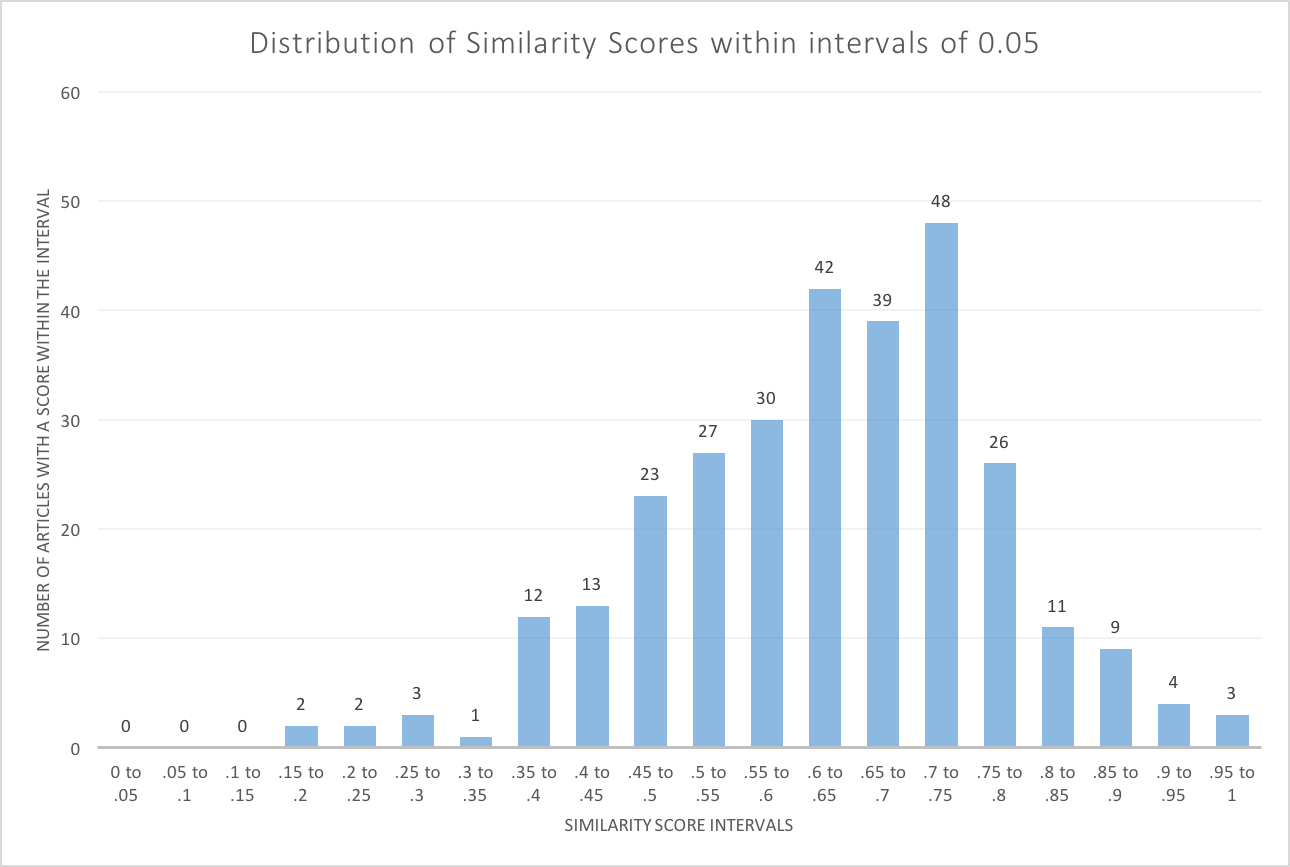
\includegraphics[width=\textwidth]{../scoreHist.png}
\caption{Distribution of scores.}
\label{scoreHist}
\end{figure*}

The distribution of scores roughly approximates a bell curve, with the center lying somewhere between 0.65 and 0.7. In fact, the average similarity score for all articles was 0.63. Notably, no articles had average similarity scores of less than 0.15, and three articles had similarity scores between 0.95 and 1.

Some tags were used for multiple articles, but there were 566 distinct tags used overall. Depending on the hypernyms produced by our algorithm for each article, these tags could be most similar to different hypernyms. For example, one article tagged as being about ``ebola'' was most similar to the hypernym ``joy,'' while a different article about ``ebola'' was most similar to the hypernym ``ill\_health.'' We computed the average number of different hypernyms matched with each distinct tag to determine whether our algorithm truly got a sense of what the article was about. On average, each tag was matched with 1.6 different hypernyms at the end of the algorithm.

\section{Discussion}

The 


% include your own bib file like this:
%\bibliographystyle{acl}
%\bibliography{acl2016}
\bibliography{acl2016}
\bibliographystyle{acl2016}

\end{document}
